\section{On binary tasks the standardized blend is a switch}\label{sec:finding2}

Eq.~\eqref{eq:blend} standardizes each branch across classes before blending, so that branches with different logit scales can be mixed.
With two classes this standardization removes everything except the sign of the prediction, and the blend can only return one branch or the other.

\paragraph{Why.}
Let $\bar z = (z - \mu)/\sigma$, with $\mu$ and $\sigma$ the mean and (population) standard deviation of the scores over the classes,
as in our implementation.
For $C = 2$ and $z_1 \neq z_2$, this gives $\bar z = (+1, -1)$ when class 1 scores higher and $(-1, +1)$ otherwise,
whatever the size of the margin.
If the anchor and the support branch agree on an image, the blend agrees with both for every $\eta$.
If they disagree, say $\bar z^0 = (+1, -1)$ and $\bar z^S = (-1, +1)$, Eq.~\eqref{eq:blend} gives
\begin{equation}
  \hat z = (1 - \eta)\,\bar z^0 + \eta\,\bar z^S = (1 - 2\eta)\,(+1, -1),
\end{equation}
which follows the anchor for $\eta < 0.5$ and the support branch for $\eta > 0.5$.
So on every test image the blended prediction equals the zero-shot prediction when $\eta < 0.5$ and the visual-only prediction when $\eta > 0.5$,
and any metric computed from predictions equals the zero-shot or the visual-only value.
How confident either branch is never enters.
At exactly $\eta = 0.5$, disagreeing branches tie and the result depends on how ties are broken.

\paragraph{Evidence.}
On BreastMNIST and PneumoniaMNIST we compared every step rule we evaluated (12 rules: PARA, shot-only, HOSO-style and nine values of the anchor-aware constant)
with zero-shot and visual only on the same draw.
In all 1,046 rule, draw and prompt-set combinations with $\eta \neq 0.5$, BAcc equals the zero-shot BAcc when $\eta < 0.5$ and the visual-only BAcc when $\eta > 0.5$.
The same holds for the oracle rows (1,128 of 1,128 including them).
Sweeping $\eta$ over a 41-point grid confirms it directly (Figure~\ref{fig:eta_curves}, blue):
in all 60 BreastMNIST runs and all 30 PneumoniaMNIST runs the z-score blend takes exactly one BAcc value for every $\eta < 0.5$ and one for every $\eta > 0.5$.
On the four-class OCTMNIST the same sweep is a genuine curve in all 60 runs.

\begin{figure}[t]
  \centering
  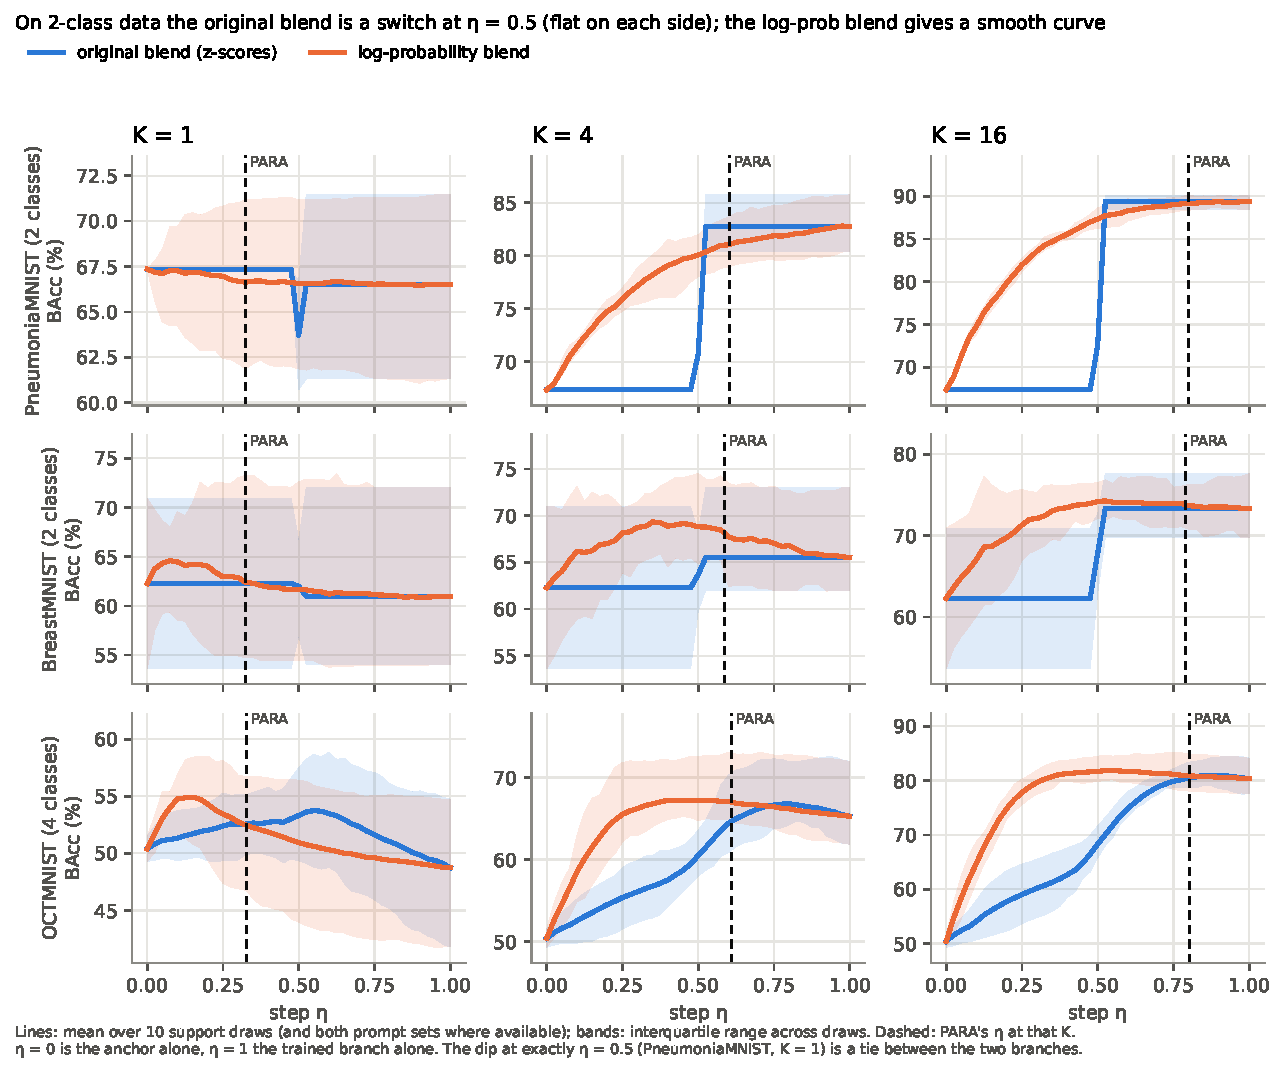
\includegraphics[width=\linewidth]{F3_eta_curves}
  \caption{BAcc as a function of the step $\eta$ for the standardized blend of Eq.~\eqref{eq:blend} (blue) and the log-probability blend of
  Section~\ref{sec:finding4} (orange), on two binary datasets and OCTMNIST.
  Lines: mean over 10 support draws and the available prompt sets; bands: interquartile range over draws.
  Dashed: PARA's step at that $K$. $\eta = 0$ is the anchor alone and $\eta = 1$ the trained branch alone.
  On the binary datasets the standardized blend is flat on each side of $\eta = 0.5$; the dip at exactly $\eta = 0.5$
  (PneumoniaMNIST, $K = 1$) is a tie between disagreeing branches.}
  \label{fig:eta_curves}
\end{figure}

\begin{table}[t]
\centering
\small
\caption{Mean BAcc (\%) over 10 support draws, averaged over prompt sets. ZS: zero-shot; z: standardized blend; lp: log-probability blend; Shot: shot-only step. Bold: best non-oracle method per row. *Oracle picks $\eta$ on the test set per draw and is not achievable.}
\label{tab:T2a_mean_bacc}
\begin{adjustbox}{max width=\linewidth}
\begin{tabular}{lrrrrrrr}
\toprule
Dataset & $K$ & ZS & Visual & PARA (z) & PARA (lp) & Shot (z) & Oracle (lp)* \\
\midrule
DermaMNIST & 1 & 21.16 & 29.70 & 26.45 & \textbf{29.91} & 28.76 & 32.24 \\
DermaMNIST & 4 & 21.16 & 45.66 & 43.98 & \textbf{46.82} & 46.09 & 47.72 \\
DermaMNIST & 16 & 21.16 & 57.68 & 57.41 & \textbf{57.94} & 57.75 & 58.62 \\
OCTMNIST & 1 & 50.40 & 48.76 & 52.56 & 52.40 & \textbf{52.72} & 56.66 \\
OCTMNIST & 4 & 50.40 & 65.28 & 64.66 & \textbf{66.98} & 66.40 & 68.72 \\
OCTMNIST & 16 & 50.40 & 80.36 & 80.49 & 80.86 & \textbf{80.97} & 82.39 \\
BloodMNIST & 1 & 14.18 & \textbf{57.76} & 34.28 & 53.09 & 43.53 & 58.12 \\
BloodMNIST & 4 & 14.18 & \textbf{82.78} & 69.39 & 81.63 & 75.80 & 82.97 \\
BloodMNIST & 16 & 14.18 & \textbf{90.73} & 88.65 & 90.57 & 89.68 & 90.81 \\
BreastMNIST & 1 & 62.28 & 60.96 & 62.28 & \textbf{62.44} & 62.28 & 70.36 \\
BreastMNIST & 4 & 62.28 & 65.50 & 65.50 & \textbf{67.81} & 65.50 & 73.17 \\
BreastMNIST & 16 & 62.28 & 73.34 & 73.34 & \textbf{73.81} & 73.34 & 76.98 \\
PneumoniaMNIST & 1 & \textbf{67.35} & 66.51 & \textbf{67.35} & 66.59 & \textbf{67.35} & 71.53 \\
PneumoniaMNIST & 4 & 67.35 & \textbf{82.75} & \textbf{82.75} & 81.03 & \textbf{82.75} & 83.41 \\
PneumoniaMNIST & 16 & 67.35 & \textbf{89.40} & \textbf{89.40} & 89.21 & \textbf{89.40} & 89.79 \\
OrganAMNIST & 1 & 25.71 & \textbf{48.97} & 37.30 & 46.79 & 41.52 & 49.59 \\
OrganAMNIST & 4 & 25.71 & \textbf{65.75} & 57.40 & 63.61 & 62.14 & 65.86 \\
OrganAMNIST & 16 & 25.71 & \textbf{81.48} & 79.74 & \textbf{81.48} & 80.59 & 81.71 \\
\bottomrule
\end{tabular}
\end{adjustbox}
\end{table}


\paragraph{Consequences for PARA.}
Because PARA's step is a fixed curve in $K$ (Section~\ref{sec:finding1}), the switch is set by the shot count alone.
On the binary datasets PARA's step never exceeds $0.347$ at $K = 1$ and is never below $0.580$ at $K = 4$,
so PARA \emph{is} zero-shot at $K = 1$ and \emph{is} visual only at $K = 4$ and $16$, on every draw
(Table~\ref{tab:T2a_mean_bacc}: on BreastMNIST, $62.28$ BAcc at $K = 1$, equal to zero-shot, and $65.50$ and $73.34$ at $K = 4$ and $16$, equal to visual only).
The shot-only schedule falls on the same side of $0.5$ at every $K$, which is why the two give identical predictions on the binary datasets in Section~\ref{sec:finding1}.

Two things follow.
First, the worst-case protection that the anchor provides is all or nothing, and which one a user gets depends only on $K$.
At $K = 1$ the switch happens to keep the anchor, which protects the worst draws:
CVaR20 is $67.35$ on PneumoniaMNIST and $62.28$ on BreastMNIST, against $53.21$ and $46.49$ for visual only.
At $K = 4$ on BreastMNIST it drops the anchor entirely: CVaR20 falls to $50.56$, the visual-only value, well below the anchor's $62.28$.
Second, no intermediate step can help, because there is no intermediate prediction.
Even the oracle can only choose a side per draw: its gains (\eg $67.65$ against $62.28$ on BreastMNIST at $K = 1$) come from picking zero-shot on some draws and visual only on others,
not from blending.
A blend that keeps each branch's confidence avoids this; Section~\ref{sec:finding4} evaluates one.
